\section*{Empirical evidence for nonnegative sparse coding in the brain}

An influential paper by Lee and Seung \cite{LeeSeung1999}
found that applying \ac{NMF} to a database of face images
yielded sparse, localized features that resembled parts of a face
(Fig.~\ref{fig:NMF|reconstruction}A).
In their case, \ac{NMF} acted on a
$F \times S$ data matrix \textbf{V},
whose rows corresponded to distinct features of the input 
(e.g., $F$ different pixels of an image)
and whose columns corresponded to different stimuli or 
observations of those features
(e.g., $S$ different images).
\ac{NMF} was used to decompose the matrix into two reduced-rank matrices
(Fig.~\ref{fig:NMF|reconstruction}, inset)
whose linear combination could be weighted such that the product of \textbf{W} and \textbf{H} provided an accurate reconstruction of \textbf{V}
(see Eq.~\ref{eqn:linear-decomposition}).

A particular image, in this case encoded by $F = 19 \times 19 = 361$ pixels
could be accurately represented by a linear combination of 
a small number ($B = 49$) of encoding variables or `basis images'
(Fig.~\ref{fig:NMF|reconstruction}A).
Such a representation is reminiscent to neural processing in \ac{IT},
an area in the ventral visual `what' stream
involved in encoding high-level object identity
\cite{BrincatConnor2004,Majaj2015},
where images of whole faces can be linearly reconstructed
using responses of approximately $200$ neurons
that each respond to a certain set of physical facial features
\cite{ChangTsao2017}.

\begin{figure}[ht]
	\centering
	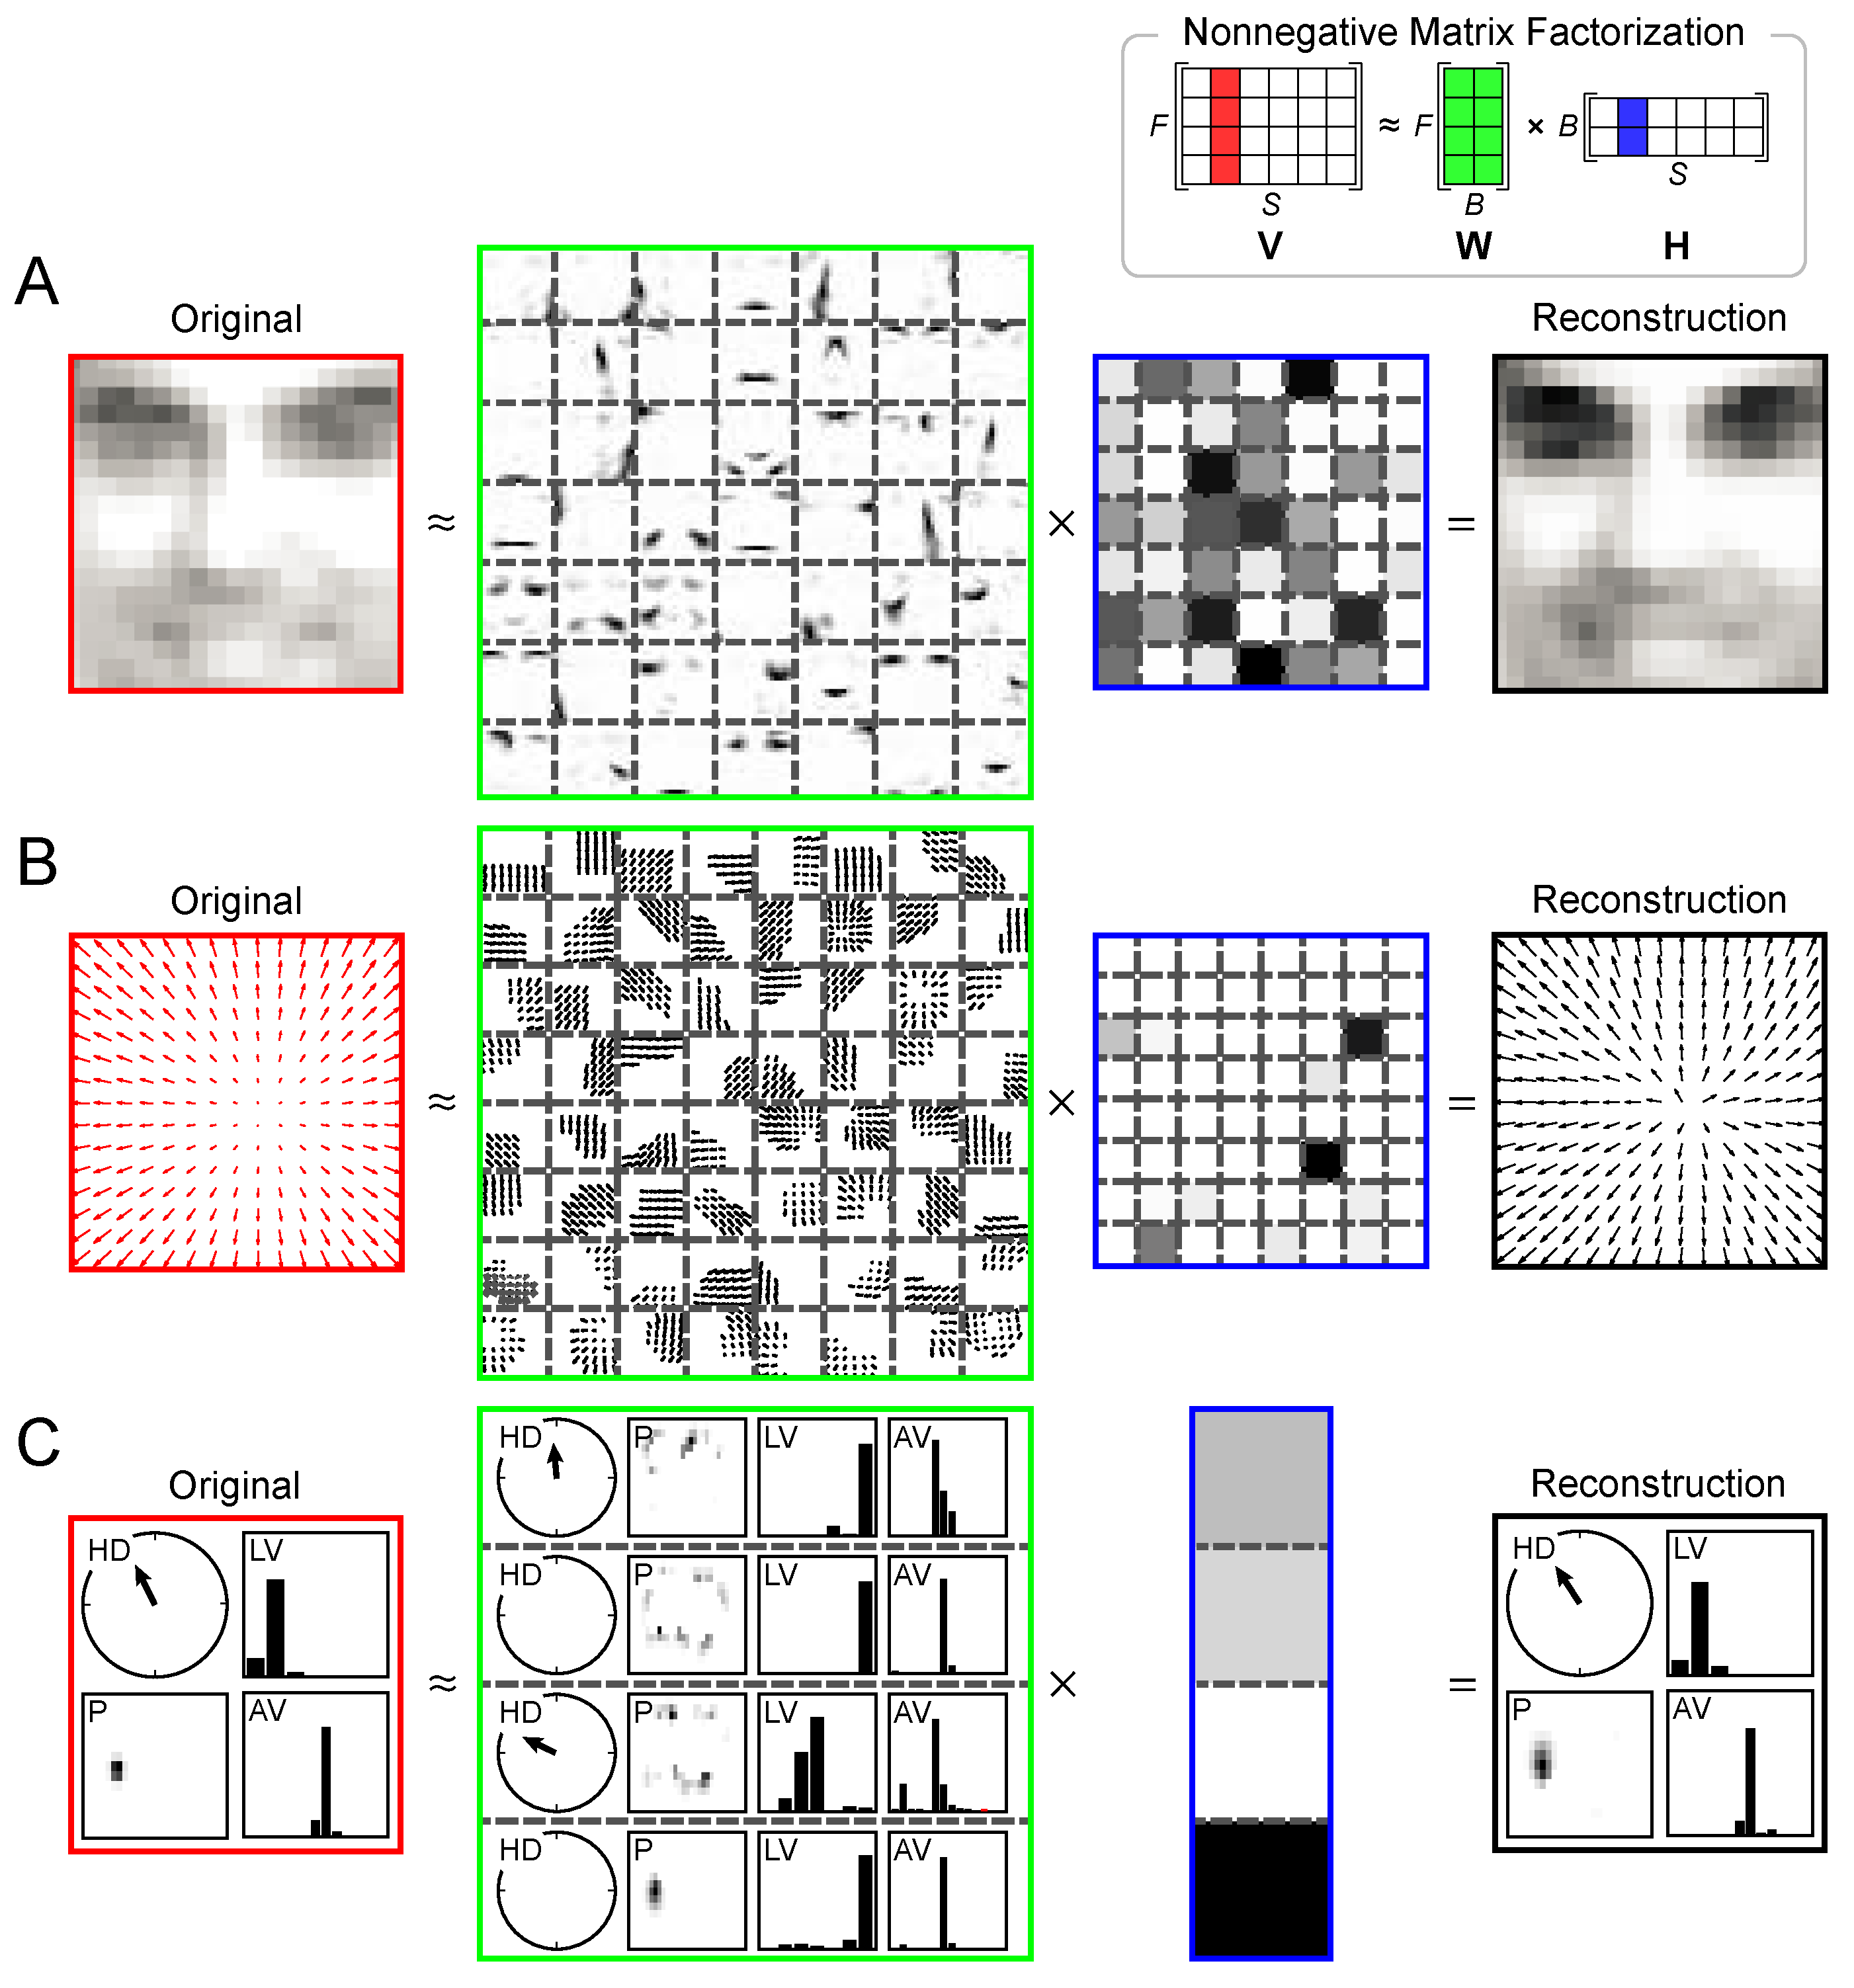
\includegraphics[width=\textwidth]{fig-rev1-reconstruction}
    \caption{Sparse and parts-based representations recovered by \ac{NMF}
             resemble receptive fields across brain regions.
             \Ac{NMF} (inset) can reconstruct a data matrix \textbf{V}
             ($F$ features x $S$ stimuli)
             from two reduced-rank matrices \textbf{W}
             (containing $B$ basis functions) and \textbf{H}
             (containing the hidden coefficients of the decomposition).
             Any individual input stimulus (i.e., column in \textbf{V}, red)
             can be reconstructed from a linear combination
             (i.e., column in \textbf{H}, blue)
             of a set of basis functions (i.e., all columns in \textbf{W}, 
             green).
         \textbf{\emph{A}},
             A facial image can be reconstructed from a sparse activation
             of simulated \acs{IT} neurons that
             preferentially respond to parts of faces
             (adapted from \cite{LeeSeung1999}).
         \textbf{\emph{B}},
             An optic flow field can be reconstructed from a sparse
             activation of model \acs{MSTd} neurons that prefer various
             directions of 3D self-translation and self-rotation
             (adapted from \cite{Beyeler2016}).
         \textbf{\emph{C}},
             A rat's 2D allocentric position and route-based direction of
             motion can be reconstructed from a sparse activation of
             model \acs{RSC} neurons that prefer an intricate combination of
             linear velocity (LV), angular velocity (AV), head direction (HD)
             and 2D position (P).
             For the sake of clarity, only the 4 most contributing hidden
             coefficients (out of 30) are shown.}
	\label{fig:NMF|reconstruction}
\end{figure}


Interestingly, such a parts-based representation is not specific to
information processing in \ac{IT};
the same principle can be extended to other areas of the visual system,
such as the \ac{MSTd},
which is part of the visual motion pathway \cite{Beyeler2016}.
Neurons in \ac{MSTd} respond to relatively large and complex patterns
of retinal motion (`optic flow'),
owing to input from direction and speed selective neurons in the \ac{MT}
(for a recent review, see \cite{Orban2007}).
Although \ac{MSTd} had long been suspected to be involved in the
analysis of self-motion,
the complexity of neuronal response properties has made it difficult
to experimentally investigate how neurons in \ac{MSTd}
might perform this function.
However, when our group
applied \ac{NMF} to 
simulated neural activity patterns whose statistical properties
resembled that of experimentally recorded \ac{MT} neurons
\cite{Beyeler2016},
we found a sparse, parts-based representation of retinal flow
(Fig.~\ref{fig:NMF|reconstruction}B)
similar to the parts-based representation of faces
encountered by Lee and Seung \cite{LeeSeung1999}.
The resulting `basis flow fields' showed a remarkable resemblance to receptive fields
of \ac{MSTd} neurons, as they responded to
an intricate mixture of
3D translational and rotational flow components
in a subset of the visual field.
As a result, any flow field possibly to be encountered 
during self-movement through a 3D environment
could be represented by only $B = 64$ simulated \ac{MSTd} neurons,
as compared to $F = 9,000$ simulated \ac{MT} input neurons.
This led to an sparse and parts-based population code,
where any given stimulus could be represented
by only a small number of simulated \ac{MSTd} neurons
\cite{Beyeler2016}.

Analogously, \ac{NSC} can explain response properties
of neurons outside the visual system, 
such as in the \ac{RSC}, an area in the posterior cingulate region
important for navigation and spatial memory \cite{Miller2014,Nelson2015,VannAggleton2009}.
Neurons in the \ac{RSC} conjunctively encode multiple variables related to the environment and one's position and movement within it
(e.g., position, head direction, linear velocity, and angular velocity),
allowing the representation of spatial features of the environment 
with respect to multiple reference frames \cite{AlexanderNitz2015}.
When our group applied \ac{NMF} to neurophysiological data from
\ac{RSC} neurons while rats ran back and forth on a W-shaped track
(for experimental details, see Supplementary Materials),
we again found a sparse and parts-based representation for behaviorally
relevant variables such as the animal's position, head direction, 
and movement direction (Fig.~\ref{fig:NMF|reconstruction}C).
Interestingly, model \ac{RSC} neurons encoded these variables with respect
to multiple frames of reference
(e.g., head direction: \textbf{allocentric reference frame},
linear velocity: \textbf{route-based reference frame}).
Once again, the dimensionality of the stimulus space was drastically reduced
from $F = 417$ input neurons to a set of $B = 30$ model \ac{RSC} neurons.

Due to its roots in efficient-coding theories of natural image processing,
there is a large body of research highlighting the role of \ac{NSC} in
visual cortex function
(e.g., \cite{Barlow1961,OlshausenField1996,Hoyer2003,BenHamed2003}).
Although there seems to be a consensus that 
information-theoretic explanations are relevant 
when investigating the early visual system,
higher-order brain areas are often considered to be specialized for
performing tasks
(e.g., recognizing objects, making decisions, navigating an environment),
rather than the efficient encoding of information.

However, more recently, 
\ac{NSC}-like computational models have found application outside visual cortex,
where they have started to provide compelling evidence that a wide variety of
neuronal response properties can be understood as an epiphenomenon
of efficient population coding based on dimensionality reduction.
Examples include elucidating the dimensions along which perceptual space
is organized in the olfactory system
\cite{MorenoBoteDrugowitsch2015,Castro2013},
the coordination of movement in the cortico-basal ganglia-thalamo-cortical loop
\cite{BarGad2000,BarGad2003_Review},
and the combined representation of allocentric and route-based 
spatial navigation cues
in retrosplenial cortex \cite{Rounds2018}.
The success of these models suggests that \ac{NSC}
might apply elsewhere in the brain, 
thus warranting further investigation.
In fact, sparse (and potentially parts-based) representations have been observed
in a wide variety of brain areas
(see Table~\ref{table:listEvidence}).
This introduces the \revise{intriguing} possibility that \ac{NSC} might
be a general principle to which \revise{many} neuronal computations adhere.
In the future, \ac{NSC} might provide a useful theoretical framework
under which to understand the often complex and nonintuitive response properties
of neurons in brain areas far removed from sensory inputs,
including the selection and integration of various task-related variables
in prefrontal cortex
\cite{Mante2013}
and the ability of premotor cortex to prepare movements without executing them
\cite{Kaufman2014}.



\begin{table}[ht]
\begin{adjustwidth}{-2.25in}{0in}
	\centering
	\caption{Nonnegative sparse coding in the brain.
    We list a group of brain regions for which there is experimental evidence of certain features associated with NSC (`X': evidence exists, `?': has yet to be investigated).
   For each brain region, the left-hand side of the table lists experimental evidence for sparse population codes and/or parts-based representations, whereas the right-hand side lists computational support that \ac{NSC}-like models can describe receptive fields or response properties within that region.}
    \def\arraystretch{1.1}
    {\setlength{\tabcolsep}{1em}
    \begin{tabular}{r|rrr|rr}
	\textbf{Brain} & \textbf{Sparse} &  \textbf{Parts-} & \textbf{Experimental} & \textbf{Modeled} & \textbf{Computational} \\
	\textbf{Area} & \textbf{code} & \textbf{based} & \textbf{evidence} & \textbf{by NSC} & \textbf{ support} \\ \hline
    Retina & X & X & \cite{Onken2016,Liu2017} & X & \cite{Onken2016,Liu2017} \\
    Visual cortex & X & X & \pbox{5cm}{\cite{OlshausenField1996,HoyerHyvarinen2002,vanHateren1998,Wachsmuth1994,FreiwaldTsao2010,ChangTsao2017,BenHamed2003}} & X & \pbox{5cm}{\cite{OlshausenField1996,Hoyer2003,Carlson2013,Hyvarinen2001,LeeSeung1999,Hosoda2009,Beyeler2016}} \\
    Auditory cortex & X & \revise{X} & \cite{Hromadka2008,rokem2006,bendor2008,Leaver2010,Terashima2013,SmithLewicki2006} & X & \cite{Martinez2015,David2007} \\
 	Olfactory cortex & X & \revise{X} & \cite{Koulakov2011,poo2009,rinberg2006,Broome2006,Castro2013} & \revise{X} & \cite{MorenoBoteDrugowitsch2015,Castro2013}  \\
 	Somatosensory cortex & X  & X & 			   \cite{Jadhav2009,oconnor2010,Crochet2011,Ramirez2014,penfield1937,hari1993,petersen2007} & X & \cite{WhitewayButts2017,Hafner2004}  \\
    Parietal cortex & ? & X & \cite{Poggio1990,PougetSejnowski1997,andersen1997multimodal,PougetSnyder2000,louie2015adaptive} & ? & ?  \\
    Retrosplenial cortex & ? & X & \cite{AlexanderNitz2015,vedder2016,mao2017} & X & \cite{Rounds2018} \\
    Prefrontal cortex & ? & ? & \cite{Mante2013,Rigotti2013,Fujisawa2008,Wei2015} & ? & ?  \\    
    Motor cortex & ? & ? & \cite{Beloozerova2003,penfield1937,GrazianoAflalo2007,Brecht2004}
    & ? & ? \\
    Hippocampus & X & ? & \cite{ThompsonBest1989,Bakker2008,myers2011pattern,rolls2013,Wixted2014,Poli2017} & ? & ? \\        
    Basal ganglia & X & ? & \cite{BarGad2003_Review,Turner2000,schwab2015} & X & \pbox{5cm}{\cite{BarGad2000,BarGad2003_Review}} \\  
	\end{tabular}}
    \label{table:listEvidence}
\end{adjustwidth}
\end{table}

In the following subsections,
we review existing experimental evidence
for sparse and parts-based representations 
in various brain areas highlighted in Table~\ref{table:listEvidence}.
Where available, we highlight \ac{NSC}-like computational models
that  successfully explain response properties of individual neurons
or have been instrumental in elucidating the dynamics at the population level.

